\chapter{BauhausBoards}\label{BauhausBoards}
Das neue Projekt bekam den Namen ``BauhausBoards''.
In einer Entwurfsphase entschied ich, wie das System aussehen und welche Funktionen es bieten sollte. Dabei flossen die Ergebnisse der Vorstudie und anderer Projekte mit ein.
\\
Als Voraussetzung sollten die Anzeigegeräte für die Türschilder weiterhin Tablets sein.
Der Entwurf wurde darauf in ein Programm umgesetzt, wobei manche geplante Funktionen geändert, entfernt oder neue hinzugefügt wurden. An manchen Stellen der Umsetzung kam es auch zu Problemen, die es zu lösen galt.
% - Ergebnisse der Vorstudie sollten enbezogen werden
% - sollte weiterhin auf Tablets als Anzeigegerät laufen
% - das was im Entwurf geplant wurde musste umgesetzt werden
% - dadurch entstanden Features
% - Während der Umsetzung traten diverse Probleme auf










\section{Entwurf}\label{Entwurf}
\subsection{Systementwurf}\label{Systementwurf}
Die Planung des Systems begann damit, die Plattform des Systems auszuwählen. Es gab die Möglichkeit eine Android-Applikation zu erstellen, die auf jedem Tablet installiert werden müsste. Dabei gäb es jedoch das Problem, dass die Nutzer auch von unterwegs mit der Anwendung interagieren sollten, wofür ein eigenständiger Server für die Datenverwaltung notwendig gewesen wäre. Außerdem müsste durch die unterschiedlichen Tablet- und Smartphone-Betriebssysteme neben Android, wie Apple IOS oder Windows Mobile, die App für jede Architektur portiert werden.
\\
Deswegen fiel die Wahl auf eine Web-Applikation. Zum Einen, weil jedes Tablet, jedes Smartphone und jeder PC Webseiten darstellen kann und es nicht nötig ist, extra eine App auf den Geräten zu installieren.
\\ \todotext{darauf eingehen, dass NetBoards auch eine Web-Applikation benutzt hat?}\\
%Zudem setzte das NetBoards Projekt ebenfalls auf eine Web-Applikation
Ein zentraler Webserver generiert eine Webseite mit allen nötigen Frontend Funktionen an, die von allen Geräten mit Web-Browser (Clients) angezeigt werden kann. Dadurch sollte sich der Programmieraufwand auf Server- und Client-Funktionen einschränken.
\\
Die Applikation sollte nicht bei jeder kleinsten Interaktion mit der Webseite diese neu laden müssen. Dies hätte einen viel zu großen Overhead erzeugt, da bei jeder Kommunikation statische Daten übertragen worden wären.
Deswegen sollte der Server nur beim ersten Aufruf das Grundgerüst der Webseite mit allen Client-Funktionen ausliefern. Ein Teil dieser Funktionen würde dann Daten nachladen oder an den Server schicken, wodurch ein dynamischer Inhalt erzeugt wird.
Dies sollte mit dem ``CRUD'' (Create, Read, Update and Delete) Prinzip realisiert werden.
Der Server wartet, nachdem er eine Seite ausgeliefert hat, auf spezifische Anfragen des Clients und liefert dementsprechend Daten aus (Read) oder ändert den Zustand der Daten (Create, Update und Delete). Zudem wird gewährleistet dieses Prinzip, dass bei Verbindungsabbrüchen die Seite auf dem Client weiter läuft und nur so lange keine Daten ändern oder nachladen kann, bis die Verbindung wieder aufgebaut wurde.
\\
Die anfallenden Daten des Systems mussten in irgend einer Form auf dem Server gespeichert werden. Die beste Methode dafür war die Nutzung einer Datenbank. Anders als bei NetBoards, wo alle Daten als JSON-Dateien auf dem Server gespeichert wurden, sah ich diese Methode als geeigneter an. Mit einer Datenbank war es möglich Relationen besser darzustellen, Konsistenz zu bewahren und Redundanz zu vermeiden. Zudem sind damit Daten zentralisiert zusammengefasst, wodurch eine bessere Suche nach bestimmten Daten möglich ist.
\\
Die Wahl des Datenbanksystems fiel auf ``SQLite''\cite{sqlite:website}, da es das am meisten verbreitete relationale Datenbanksystem der Welt ist. Es war einfach zu benutzen und hatte eine gute Dokumentation.
\\
Das Gerüst der Webseite sollte auf HTML basieren, wobei die hauptsächlichen Client-Funktionen üblicherweise in Javascript umgesetzt werden. Da die Clients viele Funktionen bieten sollten und der Server nur zum Ausliefern der Webseite und für den Datenaustausch dienen sollte, machte es Sinn für den Server ``Node.js'' zu verwenden. \quelle{Node.js ist serverseitiges Javascript basierend auf Google Chrome's V8 Javascript Engine}{nodejs:website}.
\\
\\
In der Abb. \ref{img:Systemaufbau} ist der Aufbau des Systems zusammengefasst. Auf dem Server befinden sich der Webserver und die Datenbank. Der Webserver stellt Anfragen an die Datenbank und erhält dafür entsprechende Ergebnisse zurückgeliefert.
\\
Wenn ein Client die Adresse des Servers aufruft generiert der Webserver die Webseite und sendet sie mit allen benötigten Funktionen an den Client. Solange die Seite nicht explizit neu geladen werden soll, kommuniziert der Client danach nur durch CRUD Interaktionen mit dem Server.
\\
\begin{figure}[h!]
  \centering
    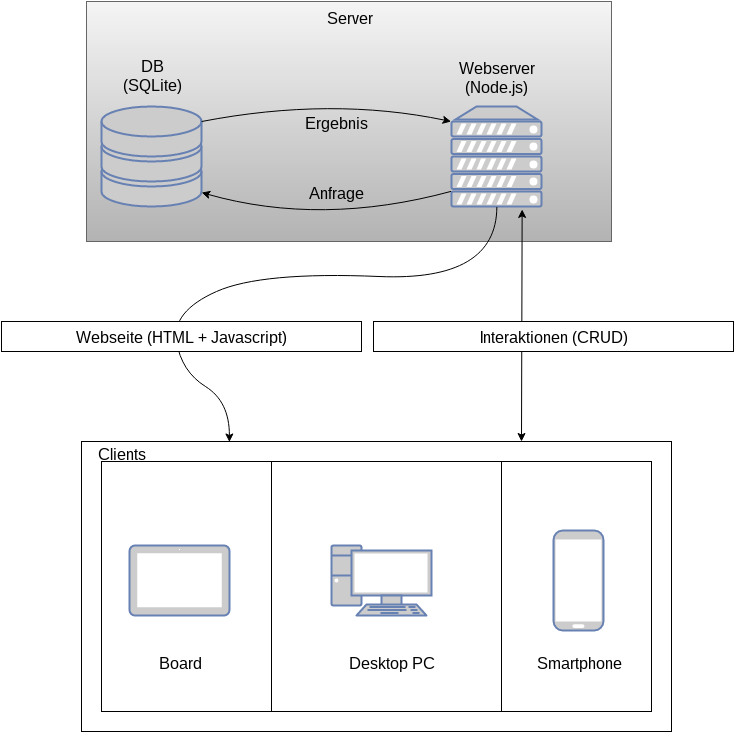
\includegraphics[width=0.8\textwidth]{./img/Systemaufbau.png}
  \caption{Bauhausboards - Systemaufbau}
  \label{img:Systemaufbau}
\end{figure}
\\
Da die Nutzer die Möglichkeit bekommen sollten, individuellen Inhalt präsentieren zu können, musste ein geeigneter Editor programmiert werden.
Damit sollte es möglich sein, einfache Zeichnungen anzufertigen, Texte zu schreiben oder Bilder hochladen zu können.
Es war wichtig, dass der Editor die Funktionen eines Whiteboards in manchen Zügen übernehmen oder möglicherweise sogar verbessern konnte.
\\
Folgende Whiteboard-Funktionen musste der Editor daher abbilden:
\begin{itemize}
  \item Zeichnen mit verschiedenfarbigen Stiften
  \item Entfernen von Zeichnungen mit einem Schwamm
  \item Anbringung von Bildern oder Ausdrücken per Magnet
  \item Neuanordnung von aufgehängten Elementen
\end{itemize}

Als Grundlage für den Editor entschied ich mich für die Javascript Bibliothek ``Paper.js''\cite{paperjs:website}.
Es ist ein Open Source Framework für die Darstellung und Manipulation von Vektorgrafiken, welches auch die Grundlage des Editors aus dem NetBoards Projekt bildete\cite{wood:2014}.

\subsection{Interface-Entwurf}\label{Interface-Entwurf}
% \begin{figure}[h!]
%   \centering
%     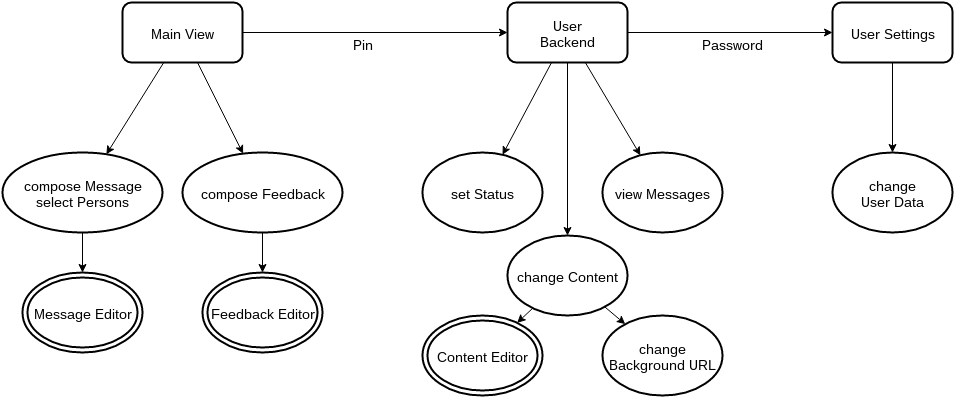
\includegraphics[width=1\textwidth]{./img/LocationsFrontend.png}
%   \caption{Bauhausboards - View Navigation Frontend}
%   \label{img:locationsFrontend}
% \end{figure}
% \begin{figure}[h!]
%   \centering
%     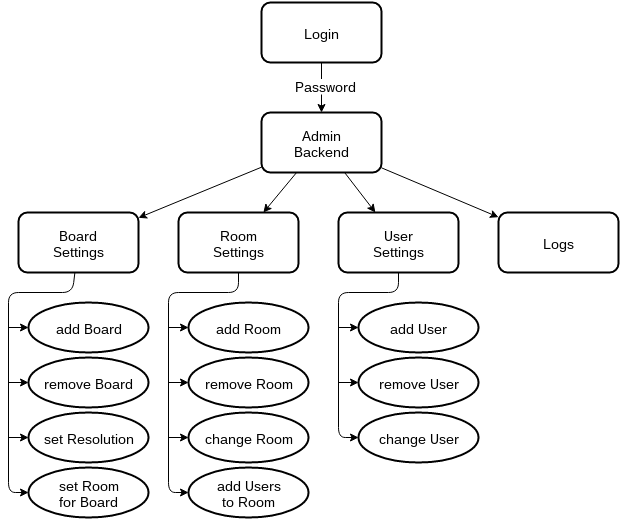
\includegraphics[width=1\textwidth]{./img/LocationsBackend.png}
%   \caption{Bauhausboards - View Navigation Backend}
%   \label{img:locationsBackend}
% \end{figure}
Da in der Vorstudie den Gästen nicht bewusst war, dass mehrere Personen auf dem Board registriert waren, was der Größe des Tablets zu verschulden war, musste der vorhandene Platz anders aufgeteilt werden.


% Sidebar
% Header

% Übernahme aus meinem Entwurf:  (Frontend)
% - Content: 2 Layers 
%   * HTML page als Hintergrund
%   * Vom Editor erstellter Content (Zeichnungen Bilder Gifs)
% - Sidebar klappt nach 10sec wieder ein
% - Wenn auf bestimmten Nutzer geklickt: dessen Content für 30sec fokused
% - Content faded über alle Nutzer
% - Gruppen Message möglich (= die Option nicht nur einer einzelnen Person eine Nachricht zu hinterlassen)
% - Sidebar ist ein und ausklappbar per swipe (besser auf Tablet) und klick
% - QR-Code, um mit Smartphone einzuscannen -> möglichkeit per smartphone Nachrichten zu hinterlassen

% Übernahme aus meinem Entwurf:  (User Backend)
% - Set Status kann einen Text setzen, der so lange angezeigt wird, wie der Nutzer es will
% - Das Backend benötigt eine Passwortauthentication
% - Change Content bietet selben Editor wie leave Message + Background layer change
% - Nutzer müssen Möglichkeit bekommen Nachrichten einzusehen
% - Ungelesene Nachrichten sollen gehighlighted werden
% - Backendfunktionen nur für den Nutzer, der sich authentisiert hat

% Übernahme aus meinem Entwurf:  (Admin Backend)
% - Nur für Nutzer mit Adminstatus zugänglich
% - Statistics
% - Add, Change, Remove Users, Rooms, Boards
% - 'sind sie sicher' prompts
% - Logs, um sich den Inhalt des Raumes anzusehen


% Screen
% Sidebar

% Da Screen zu klein war in der Vorstudie den gästen nicht bewusst, dass sich zwei leute den Raum teilten
% -> Teilen des Screens für alle Nutzer des Raumes? nein!
% -> Jeder Nutzer sollte den Ganzen Screen für die ANzeige ihres Contents bekommen
% -> Deswegen Switch der Contentseite über alle Nutzer im Raum nach bestimmter Zeit + Feste Boardgröße ohne Scroll (Zumindest auf dem Tablet)
% Statusmeldungen für jeden Nutzer
% -> jeder Nutzer sollte die Möglichkeit bekommen einen Status für sich setzten zu können, der aus einem kurzen Text (wie: bin Mittag essen oder bin im Meeting) und die angepeilte dauer des Status (~ bis 12:00)
% Kommunikation der Besucher mit den Besitzern
% -> es sollte den Besuchern möglich sein mit den Besitzern des Raumes in verbindung zu treten
% -> Nachrichtensystem erstellt
% -> Besucher sollen einem, mehreren oder allen Nutzern des Raumes eine Nachricht hinterlassen können
% -> Die Besitzer sollen darauf eine Email bekommen, dass jemand an ihr Board geschrieben hat (Mit Inhalt der Nachricht)
%Aufbau der Seite
% - mehrere Personen in Raum --> wie realisieren?
% - switch durch alle angemeldeten User im Raum
% - Jeder hat eigenen Content
% - Nutzer wollen vllt nur eine Person in einem Raum ansprechen oder mehrere oder vllt sogar alle
% - Nutzer im Raum müssen in irgend einer Weise darüber informiert werden, dass sie eine Nachricht erhalten haben --> mail / app
% - Administrator der Applikation muss die Möglichkeit haben neue Nutzer, neue Räume und neue Boards zu erstellen und initialisieren
% - Zu Studienzwecken muss der Administrator zudem in der Lage sein alle Nachrichten und erstellte COntents auswerten zu können
% - Nutzer die Vorbei gehen sollen in irgend einer weise Feedback senden können (in Vorstudie hat sich gezeigt, dass niemand auf die daneben aufgehangenen Zettel etwas schreiben wollte - deshalb direktes Feedback per app)
% - Benutzer in den Räumen müssen die Möglichkeit haben alle Nachrichten, die sie erhalten haben einsehen zu können
% - Neue Nachrichten müssen besonders gekennzeichnet sein
% - Zudem sollen sie Ihre Pinnwand anpassen können
% - Sie sollen Skizzen machen können, Bilder und Gifs hochladen und Webseiten als Hintergrund laden können
% - Um schnell einen Status zu setzen, quasi wenn man schnell weg muss und an seinem Board vorbei geht, soll zum Authentisieren des Nutzers ein 4 Stelliger PIN genutzt werden. Der Nutzer soll angeben, welcher der registrierten Nutzern des Raumes er ist und dazu seinen PIN eingeben. Wenn er das getan hat kann er einen Status setzen oder sich als Verfügbar/Nicht Verfügbar kennzeichnen
% - Sie sollen einen Status setzen können, um vorbeigehende Nutzer darüber zu Informieren, was sie jetzt zur Zeit machen, ob sie grade im Büro sind, nur kurz essen, den halben oder ganzen Tag nicht da sind oder im Labor anzutreffen sind
% - Zudem sollen sie die möglichkeit bekommen sich als nicht anwesend markieren zu können, damit Gäste, die auf die Boards schauen schnell sehen, wer da ist und wer nicht
% - Nutzer im Raum, die gern Twitter benutzen sollen die öglichkeit bekommen ihren TwitterAccount anzugeben, damit ihr letzter tweet auf ihrer Pinnwand angezeigt werden kann
% - Nutzer im Raum sollen zudem Ihre ganzen Daten ändern können (Name, Beschreibung, Mail, ProfilePic, PAsswort, PIN, ...) Dazu ist aber das Passwort des Nutzers erforderlich

% - Grundüberlegung des Seitenaufbaus
% - erster Entwurf der Seitenstruktur als Bild
% - Routen im ganzen System
%  * Frontend
%    # Main View
%    # Message View
%    # Feedback View
%    # User Backend View
%      + Status
%      + Content
%      + Received Messages
%      + User Settings
%  * Backend
%    # Boards
%      + add
%      + del
%      + set Room
%      + set Resolution
%    # Rooms
%      + add
%      + del
%      + change name/descr
%      + manage room users
%    # Users
%      + add
%      + del
%      + change User
%    # Logs
%      + Contents
%      + Messages
%      + Feedbacks
% - Sidebar zum Navigieren
% - Überlegung zur Auslagerung des Admin Backends
% - Hinleitung zur Umsetzung

\subsection{Datenbankentwurf}\label{Datenbankentwurf}
% \begin{figure}[h!]
%   \centering
%     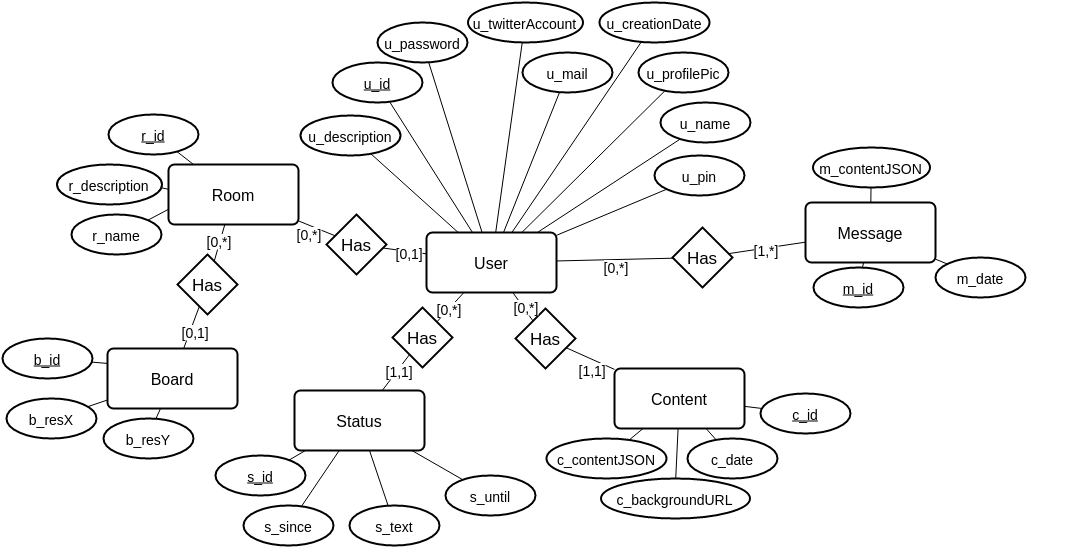
\includegraphics[width=1\textwidth]{./img/ER01.png}
%   \caption{Bauhausboards - Datenbankentwurf}
%   \label{img:ER01}
% \end{figure}
% 
%Aufbau der Datenbank
%SQLITE anstelle von MONGODB
%- kein traditionelles Relationales Schema
%- Mongodb hätte jedoch direkt JSON results
%- Für kleines Umfeld ist SQLITE auch akzeptabel
%- alternativen wären: mysql
%- nodejs hat aber auch ein npm repo für sqlite
% - Um die Daten Zentral auf dem Server verwalten zu können musste eine Datenbank eingerichtet werden
% - Hierbei bestand die Frage, ob klassische Relationale DB oder dokument-orientierte DB
% - dokument-orientiert vorteile wegen JSON strings, nachteile: keine Relationen, alles in Strings, starkes umdenken erforderlich für NUtzer mit Kenntnis über Relationale DBs
%- Relationale DB wird genutzt (SQLITE), damit lassen sich Zusammenhänge leicht deklarieren, SQLite ist zudem lightweight und wird für nicht ganz so aufwändige Schemata genutzt
% - zum Schema: (ER Diagramm hier einfügen)
%   * User Tabelle
%     zum Speichern der Nutzerdaten
%     auf typen eingehen (warum Name und Descr. nur 30 Zeichen, warumn PIN und PW 64char - SHA256 hex string)
%   * Room Tabelle
%     name und description (zur Kennzeichnung von Physikalischen Räumen)
%   * Roomusers Tabelle
%     Nutzer können sich in mehreren Räumen anmelden
%   * Board Tabelle
%     resolution und roomID
%     jedes Board hat eine andere Auflösung - um den Kontent auf jedem Board korrekt anzeigen zu können, muss die Auflösung des Boards ausgelesen werden, zudem hängt jedes Board nur vor einem Raum und kann dementsprechend auch nur einem Raum zugewiesen werden
%   * Content Tabelle
%     wenn ein Nutzer Kontent erzeugt oder ändert wird ein neuer Eintrag erzeugt, um jegliche Änderung später auswerten zu können
%     Dazu gehört wann die änderung statt fand, was der neue Content ist und was als Background URL eingestellt ist
%   * message Tabelle
%     jedes mal wenn ein Nutzer auf einem Board eine Nachricht für einen oder mehrere Nutzer erstellt wird ein neues Element angelegt
%     Zeit und INhalt der Nachricht werden hier gespeichert, die Relation mit USer wird über eine dritte Tabelle realisiert
%   * msgTo Tabelle
%     hier werden die PS von User und Message zusammengefasst. Zudem wird hier angegeben, ob der entsprechende Nutzer diese Nachricht schon gelesen hat und ein Token wird generiert, wodurch der Nutzer diese Nachricht direkt aufrufen kann, ohne sich vorher anmelden zu müssen
%   * status Tabelle
%     hier wird der Status der Nutzer gespeichert, jedes Mal wenn der Nutzer einen neuen Status angibt, wird ein neuer Eintrag erzeugt. Nur der neuste Status ist gültig
%     gespeichert wird die erstellzeit, endzeit, der statustext und der dazugehörige Nutzer
%   * feedback Tabelle
%     hier werden alle feedback drafts abgelegt mit timestamp





















\section{Umsetzung}\label{Umsetzung}
Größter Part: Die Komplette Umsetzung im Detail

% - NodeJS
%   * da frontend größtenteils mit Javascript laufen sollte und ich mich auf eine einheitliche programmiersprache festlegen wollte
%   * Server liefert nur Grundaufbau und JS der Seite aus
%   * Ansonsten wartet er nur auf CRUD befehle um den datenbank state zu ändern oder zu erwiedern
%   * Express app für mvc policy
%   * banquo           -- dafür da umhtml seiten zu einem image zu rendern
%    body-parser       -- middleware für express zum parsen des bodys ??? was macht das ding??
%    canvas            -- teil von paperjs
%    cookie-parser     -- cookie tool
%    crypto-js         -- crypto library für passwort hashes
%    debug             -- debug tool
%    emailjs           -- tool zum senden von mails
%    express           -- mvc framework
%    express-session   -- session tool for express
%    jade              -- template engine
%    jquery            -- JS DOM manipulation tool
%    jquery-touchswipe -- small tool to enable a swipe gesture
%    moment            -- JS time tool
%    morgan            -- http request logger
%    nib               -- middleware for stylus
%    paper             -- canvas manipulation tool
%    serve-favicon     -- express enable favicon
%    sqlite3           -- database api
%    stylus            -- css generator
%    twitter           -- twitter api tool
%    uuid              -- session uuid generator
% - Frontend: HTML mit Javascript und JQuery zum Dom-manipulieren
%   * Webseite wird nur einmal geladen, um damit alles nötige zu holen
%   * Dynamischer Content wird per ajax vom Server geholt
%   * bei verbindungsabbrüchen werden bestimmte states gehalten und andere sind durch inconnectivität nicht möglich
%   
%
%Packages:
%- Express
%- SQLite
%  * warum SQLite anstelle von MongoDB (relational vs dokument-orientiert)
%- PaperJS
%- crypto-JS for SHA256 password/pin hashing
%- ....
%
%Server
%Struktur der Webseite
%Editor
% -> Was ist besser gegenüber den Funktionen, die er anfangs haben sollte?
% -> Privacy
% -> Nur als Framework vorhanden -> Interface musste selbst erstellt werden
% -> Voraussetzung: HTML5 Canvas Element
%Backend
%Design CSS
%Bootstrap
%Javascript Code??

% Emailtoken
% wenn eine Nachricht an einen Besitzer abgeschickt wird, wird ein Token generiert, der mit der Nachricht verbunden wird, dieser Token wird dann in der url in der benachrichtigungsmail mitgeschickt und ruft beim Aufruf der der url die Nachricht ab

% Sessions
% Ajax zur realisierung von CRUD









\section{Features}\label{Features}
Alle Features des Boards\\
\\
% Unterschied zu Hermes / NetBoards
% jeder user hat eigene Pinnwand weil tablet resolution nicht so groß und dadurch wenig platz, mach keinen sinn für alle nutzer im raum nur eine pinnwand zu bieten (vergleich NetBoards) - switch betweeen them
%so ein bischen gestalten, wie das how to pdf
%Editor:
%Drag and Drop Images - URL wird geholt und ein neues Image wird erzeugt
% imgUR API
%Pen
%text
%Stroke Size
%Color
%farbe von pen und text elementen ändern
%
%Auswahlwerkzeug:
%selektierung von einzelnen Objekten
%selektierung von mehreren objekten mit bounding box
%Popup
%löschen von markierten elementen
%Layering
%Kopieren
%Translation der Objekte in Bounding Box
%Scale der Objekte in Bounding Box
%Rotation der Objekte in der Bounding box
%Eraser Tool
%UNDO/REDO
%Image Upload
%Image Drag and Drop
%Gif Layer Support
%
%Twitter API für den letzten Tweet eines bestimmten Nutzers 
%
%Client Sessions
%mit npm plugin express-sessions serverseitig
%cookie ID client seitig
%caching of content for disconnects
%N/A marking of user image
%status set
%background layer
%nachrichten schreiben >> mail versenden mit unique token >> nachricht content direkt lesen mittels token
%  * nachricht an 1, 1+ oder alle im raum schicken
% feedback: hat einfach nur den editor

%Backend
% logs, user, room, board administration


















\section{Probleme}\label{Probleme}
Die Probleme, auf die ich während der Arbeit gekommen bin\\
%Editor:\\
%- Gif Layer Hack\\
%- Scale Problem\\
%- Stroke Size Problem\\
%Problem: Desktop Version dimensions
%- die Auflösung auf dem Desktop ist größer als auf dem Tablet
%- content, der auf dem Desktop weiter rechts/weiter unten erstellt wird, verschwindet auf dem tablet :(
%- Lösungsansätze:
%  # Canvas resize auf größeren Auflösungen
%  # anzeige von linien, wie es auf dem tablet angezeigt wird
%Problem Header
%- durch horizontale ausrichtung der tablets ist der Platz des header zu groß und wird verschwendet
%- wenn nur userimage, username, status, description usw angezeigt werden muss
%- Lösung: absolutes header div, welches oben rechts in der ecke ist
%  # content hat dadurch tatsächlich die größe des tablets
%  # platz wird nicht so stark verschwendet
%  # "toter winkel" oben rechts in den raw datas der images
%- die ganze css datei muss angepasst werden, da positionen und größen relativ zum header gesetzt waren
%- random server deadlock --> restart script
%- Message Email mit image direkt in der NAchricht im HTML als <img> element ging nicht, da  cross origin resource sharing(CORS) nicht aktiviert ist (origin-clean flag false) deswegen geht die Funktion .toDataURL("image/png") nicht
%   * Zudem ist es schwer in der mail ein paperJS project in ein canvas einzubinden
%   * deswegen die Überlegung beim erstellen der message das canvas objekt direkt zu exportieren